
Let
\begin{align}
    &\vec{A} = \myvec{1\\5},\\
    &\vec{B} = \myvec{2\\3},\\
    &\vec{C} = \myvec{-2\\-11}
\end{align}
and 
\begin{align}
    \vec{M}=\myvec{\vec{B-A} & \vec{C-A}}^T
\end{align}
If $rank(\vec{M}) = 1$, the points are collinear.  The rank of a matrix is the number of nonzero rows left after doing row operations.  In this problem, 
\begin{align}
    \vec{M} = \myvec{1 & -2\\-3 & -16}\xleftrightarrow {R_2\leftarrow -\frac{R_2}{3}-R_1}\myvec{1 & -2\\0 & \frac{22}{3}}
    \\
    \implies rank(\vec{M}) = 2
    \end{align}
Therefore, the points are not collinear.  This is verified in Fig. \ref{aug/2/7/plot}.

\begin{figure}[!ht]
    \centering
    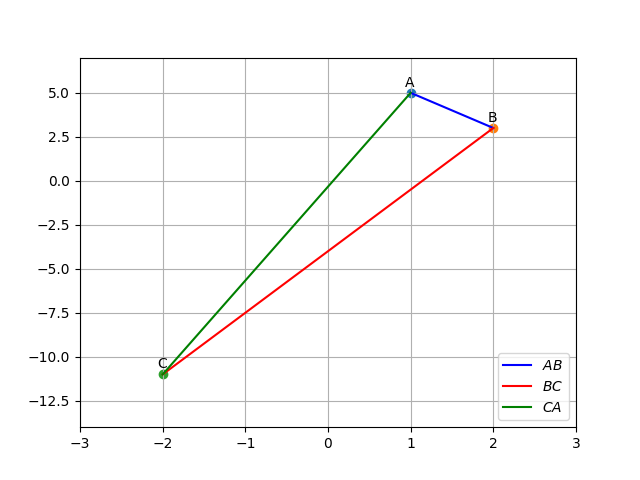
\includegraphics[width=\columnwidth]{solutions/aug/2/7/figure/figure.png}
    \caption{Plot of the points}
    \label{aug/2/7/plot}
    \end{figure}
